\begin{defi}[Operador de Laplace]
Seja $f$ uma função duplamente derivável de valores reais no espaço euclidiano $\mathbb{R}^n$. O \textbf{operador de Laplace} (também conhecido como Laplaciano), denotado por $\Delta$ ou $\nabla^2$, é definido como o divergente do gradiente:
\begin{equation}
\Delta f = \nabla^2 f = \nabla \cdot (\nabla f) = \text{div} (\text{grad f})
\end{equation}
\end{defi}

O \textbf{operador de Laplace-Beltrami} é assim denominado no contexto de geometria diferencial por também operar sobre funções definidas em subvariedades no espaço euclideano.

\begin{defi}[Coordenadas diferenciais]
	Seja uma malha triangular de $n$ vértices caracterizada por $\mathcal{M} = (V, E, F)$, em que $V, E, F$ são, respectivamente, os conjuntos de seus vértices, arestas e faces, e cada vértice $\mathbf{v}_i \in V$ possui uma coordenada cartesiana dada por $\mathbf{v}_i = (x_i,y_i,z_i)$. \textbf{Coordenadas diferenciais} (também conhecidas como $\mathbf{\delta}$\textit{-coordenadas}) de $\mathbf{v}_i$ são definidas como a diferença entre a coordenada cartesiana e o centro de massa de seus vizinhos imediatos na malha:
	
	\begin{equation}
	\mathbf{\delta}_i = (\mathbf{\delta}_i^{(x)}, \mathbf{\delta}_i^{(y)}, \mathbf{\delta}_i^{(z)}) = \mathbf{v}_i - \frac{1}{d_i} \sum_{j \in N(i)} \mathbf{v}_j,
	\label{eq_delta}
	\end{equation}
	
	\noindent em que $N(i) = \{j\ |\ (i,j) \in E$\} (ou seja, o conjunto dos vértices adjacentes a $i$) e $d_i = |N(i)|$ é o número dos vizinhos imediatos de $i$ (grau de $i$).
\end{defi}

As $\mathbf{\delta}$-coordenadas podem ser vistas como a discretização do operador contínuo de Laplace-Beltrami, caso a malha $\mathcal{M}$ seja a aproximação linear por partes de uma superfície suave. Pode-se denotar o vetor de coordenadas diferenciais em um vértice $v_i$ como

\begin{equation}
\mathbf{\delta}_i = \frac{1}{d_i} \sum_{j \in N(i)} (\mathbf{v}_i - \mathbf{v}_j)
\end{equation}

\noindent em que este somatório é a discretização da seguinte integral:

\begin{equation}
\frac{1}{|\gamma|} \int_{\mathbf{v} \in \gamma} (\mathbf{v}_i - v) dl(\mathbf{v}))
\end{equation}

\noindent onde $\gamma$ é uma superfície simples e fechada em torno de $\mathbf{v}$ e $|\gamma|$ é o comprimento de $\gamma$. Sabe-se, de geometria diferencial, que

\begin{equation}
\lim_{|\gamma| \rightarrow 0} \frac{1}{|\gamma|} \int_{\mathbf{v} \in \gamma} (\mathbf{v}_i - \mathbf{v}) dl(\mathbf{v}) = -H(\mathbf{v}_i)\mathbf{n}_i
\end{equation}

\noindent em que $H(\mathbf{v}_i)$ é a curvatura média em $\mathbf{v}_i$ e $\mathbf{n}_i$ é o vetor normal à superfície.

Assim, a direção do vetor de coordenadas diferenciais aproxima-se à direção normal e sua norma aproxima a quantidade proporcional à curvatura média local. De maneira resumida, isto significa que as $\mathbf{\delta}$-coordenadas encapsulam a forma da superfície local. %, como ilustra a figura \ref{fig:coordDif}.

% \begin{figure}[htb]
% 	\centering
% 	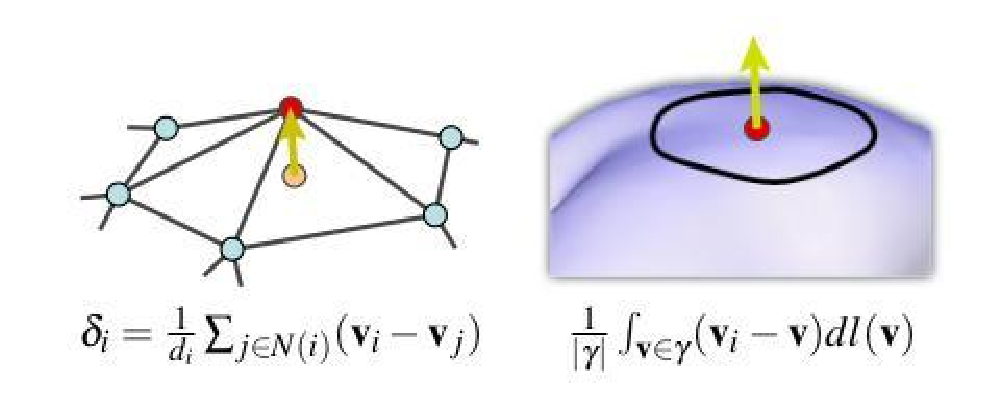
\includegraphics[width=.7\linewidth]{imagens/cap4/difcoord.eps}
% 	\caption{O vetor da coordenada diferencial em um vértice aproxima a forma local superfície \cite{sorkine2006}}
% 	\label{fig:coordDif}
% \end{figure}

A transformação do vetor de coordenadas cartesianas absolutas ao vetor das $\mathbf{\delta}$-coordenadas, descrita na equação \ref{eq_delta}, também pode ser representada em forma de matriz. Seja $A$ a matriz de adjacências da malha, descrita por:

\begin{equation}\label{eqMatAdj}
A_{ij} = \begin{cases}
1&(i, j) \in E\\
0&\text{caso contrário.}
\end{cases}
\end{equation}

\noindent e $D$ matriz diagonal tal que $D_{ii} = d_i$ (grau do vértice $i$). A matriz transformação de coordenadas absolutas para as coordenadas relativas é:

\begin{equation}
L = I - D^{-1}A.
\end{equation}

Porém, é mais conveniente (e computacionalmente eficiente) utilizar a versão simétrica $L_s$ da matriz $L$, definida por:

\begin{equation}\label{eqMatLaplaciana}
L_s = DL = D - A
\end{equation}

\noindent em que cada célula pode ser calculada da seguinte forma:

\begin{equation}
(L_s)_{ij} = \begin{cases}
d_i&i=j\\
-1&(i, j) \in E\\
0&\text{caso contrário.}
\end{cases}
\end{equation}

A matriz $L_s$ é denominada \textit{Laplaciano topológico} da malha $\mathcal M$. Por exemplo, para a seguinte malha, descrita pela figura \ref{fig:origmesh}:

\begin{figure}[ht!]
	\centering
	\includegraphics[width=.6\linewidth]{imagens/cap4/grafo.eps}
	\caption{Uma malha triangular com posições cartesianas descritas no $\mathbb{R}^2$}
	\label{fig:origmesh}
\end{figure}

\noindent têm-se as seguintes matrizes $A$ de adjacências e diagonal $D$:

$$A = \begin{pmatrix}
0 & 0 & 1 & 1 & 0 & 0 & 1 & 1 & 1\\
0 & 0 & 0 & 0 & 1 & 1 & 0 & 1 & 0\\
1 & 0 & 0 & 1 & 0 & 1 & 0 & 1 & 0\\
1 & 0 & 1 & 0 & 0 & 0 & 0 & 0 & 1\\
0 & 1 & 0 & 0 & 0 & 0 & 1 & 1 & 0\\
0 & 1 & 1 & 0 & 0 & 0 & 0 & 1 & 0\\
1 & 0 & 0 & 0 & 1 & 0 & 0 & 1 & 1\\
1 & 1 & 1 & 0 & 1 & 1 & 1 & 0 & 0\\
1 & 0 & 0 & 1 & 0 & 0 & 1 & 0 & 0
\end{pmatrix}\ \ D = \begin{pmatrix}
5 & 0 & 0 & 0 & 0 & 0 & 0 & 0 & 0\\
0 & 3 & 0 & 0 & 0 & 0 & 0 & 0 & 0\\
0 & 0 & 4 & 0 & 0 & 0 & 0 & 0 & 0\\
0 & 0 & 0 & 3 & 0 & 0 & 0 & 0 & 0\\
0 & 0 & 0 & 0 & 3 & 0 & 0 & 0 & 0\\
0 & 0 & 0 & 0 & 0 & 3 & 0 & 0 & 0\\
0 & 0 & 0 & 0 & 0 & 0 & 4 & 0 & 0\\
0 & 0 & 0 & 0 & 0 & 0 & 0 & 6 & 0\\
0 & 0 & 0 & 0 & 0 & 0 & 0 & 0 & 3
\end{pmatrix}$$

\noindent que geram o seguinte laplaciano topológico $L_s$:

$$L_s = \begin{pmatrix}
5 & 0 & -1 & -1 & 0 & 0 & -1 & -1 & -1\\
0 & 3 & 0 & 0 & -1 & -1 & 0 & -1 & 0\\
-1 & 0 & 4 & -1 & 0 & -1 & 0 & -1 & 0\\
-1 & 0 & -1 & 3 & 0 & 0 & 0 & 0 & -1\\
0 & -1 & 0 & 0 & 3 & 0 & -1 & -1 & 0\\
0 & -1 & -1 & 0 & 0 & 3 & 0 & -1 & 0\\
-1 & 0 & 0 & 0 & -1 & 0 & 4 & -1 & -1\\
-1 & -1 & -1 & 0 & -1 & -1 & -1 & 6 & 0\\
-1 & 0 & 0 & -1 & 0 & 0 & -1 & 0 & 3
\end{pmatrix}$$

Com isso, pode-se calcular as coordenadas diferenciais referentes ao eixo-x da seguinte forma:

\begin{equation}
L_s \mathbf{x} = \mathbf{\delta}^{(x)}
\end{equation}

\noindent e isto é feito de forma análoga para os outros eixos, a depender da dimensão da malha em análise.

Já foi mostrado como obter as coordenadas diferenciais a partir das coordenadas absolutas e do laplaciano topológico. Agora será analisado como se recuperar as coordenadas absolutas.

As $\delta$-coordenadas são invariantes à translação. Isto ocorre pois caso a malha $\mathcal{M}$ seja transladada de acordo com um vetor $u$ gerando novos vértices $v_i'$, tem-se:

\begin{align*}
L(\mathbf{v}_i') &= \sum_{j \in N(i)} w_{ij} (\mathbf{v}_i' - \mathbf{v}_j')\\ 
 &= \sum_{j \in N(i)} w_{ij} ((\mathbf{v}_i + \mathbf{u})  - (\mathbf{v}_j + \mathbf{u}))\\ 
 &= \sum_{j \in N(i)} w_{ij} (\mathbf{v}_i - \mathbf{v}_j) = L(\mathbf{v}_i)
\end{align*}

Assim, as matrizes $L$ e $L_s$ são singulares, e $\mathbf{x} = L_s^{-1} \mathbf{\delta}^{(x)}$ é indefinido. Mais que isso, como cada componente da malha possui um grau de liberdade de translação, tem-se que $rank(L) = n - k$, em que $k$ é o número de componentes. Para que seja possível restaurar as coordenadas absolutas, é necessário que o sistema linear seja \textit{full-rank} - e isto pode ser alcançado adicionando restrições para fixar a localização de alguns vértices.

Por simplicidade de notação, suponha que sejam fixados a localização de $m$ vértices com índices $P = \{1, 2, \cdots, m\}$, em que são conhecidas as localizações $c = \{\mathbf{v}_j\ |\ j \in P\}$. Serão adicionadas restrições do tipo:

$$\mathbf{v}_j = \mathbf{c_j}, \forall\ j \in P$$

Com a denotação matricial, o novo sistema linear será:

\begin{equation}\label{eq:sisrecover}
\left( \frac{L}{\omega I_{m \times m} | 0} \right) \mathbf{x} = \begin{pmatrix}
\delta^{(x)}\\
\omega\ c_{1:m}^{(x)}
\end{pmatrix}
\end{equation}

\noindent e o mesmo vale para os outros vetores de coordenadas. Com a utilização do vetor $\omega > 0$, cada restrição pode possuir um peso diferente, que pode ajustar a importância e relevância de cada vértice.

De forma gráfica, para facilitar a visualização do sistema:

\begin{center}
	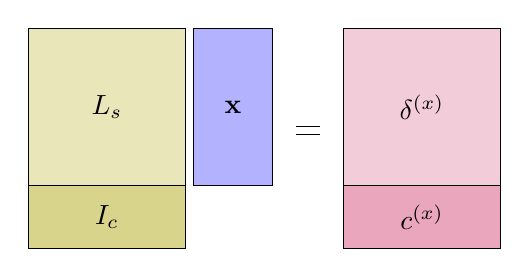
\begin{tikzpicture}
	\filldraw[fill=olive!20!white, draw=black] (0,0) rectangle node{$L_s$} (2,2);
	\filldraw[fill=olive!35!white, draw=black] (0,0) rectangle node{$I_c$} (2,-0.8);
	\filldraw[fill=blue!30!white, draw=black] (2.1,0) rectangle node{$\mathbf{x}$} (3.1,2);
	\draw (3.4, 0.65) -- (3.7, 0.65);
	\draw (3.4, 0.75) -- (3.7, 0.75);
	\filldraw[fill=purple!20!white, draw=black] (4,0) rectangle node{$\delta^{(x)}$} (6,2);
	\filldraw[fill=purple!35!white, draw=black] (4,0) rectangle node{$c^{(x)}$} (6,-0.8);
	\end{tikzpicture}
\end{center}

\noindent neste caso, $I_c$ é a matriz identidade $m \times m$, com zeros à direita (e foi fixado $\omega = 1$ por simplicidade).

A matriz dos coeficientes em \ref{eq:sisrecover} é denominada $\tilde{L}$. Por mais que o sistema tenha mais equações que incógnitas, ele é \textit{full-rank} e possui uma única solução com a utilização do método dos mínimos quadrados:

\begin{equation}\label{eq:leastsqrsol}
\mathbf{\tilde{x}} = \mathop{\mathrm{argmin}}_x \left( \lVert L \mathbf{x} - \delta^{(x)} \rVert^2 + \sum_{j \in C} \omega^2 \lvert x_j - c_j \rvert^2  \right)
\end{equation}

Então, por exemplo, para a mesma malha mostrada anteriormente, caso seja fixada a localização dos vértices $1$ e $5$ (como mostrado na figura \ref{fig:fixedmesh}) temos:

\begin{figure}[ht!]
	\centering
	\includegraphics[width=.6\linewidth]{imagens/cap4/grafofixado.eps}
	\caption{Uma malha triangular com os pontos $1$ e $5$ fixados}
	\label{fig:fixedmesh}
\end{figure}

\noindent e é formada a seguinte matriz $\tilde{L}$:

$$\tilde{L} = \begin{pmatrix}
5 & 0 & -1 & -1 & 0 & 0 & -1 & -1 & -1\\
0 & 3 & 0 & 0 & -1 & -1 & 0 & -1 & 0\\
-1 & 0 & 4 & -1 & 0 & -1 & 0 & -1 & 0\\
-1 & 0 & -1 & 3 & 0 & 0 & 0 & 0 & -1\\
0 & -1 & 0 & 0 & 3 & 0 & -1 & -1 & 0\\
0 & -1 & -1 & 0 & 0 & 3 & 0 & -1 & 0\\
-1 & 0 & 0 & 0 & -1 & 0 & 4 & -1 & -1\\
-1 & -1 & -1 & 0 & -1 & -1 & -1 & 6 & 0\\
-1 & 0 & 0 & -1 & 0 & 0 & -1 & 0 & 3\\
1 & 0 & 0 & 0 & 0 & 0 & 0 & 0 & 0\\
0 & 0 & 0 & 0 & 1 & 0 & 0 & 0 & 0
\end{pmatrix}$$

\noindent e a recuperação das coordenadas absolutas com relação ao eixo-x é feita a partir da resolução do seguinte sistema linear:

$$\begin{pmatrix}
5 & 0 & -1 & -1 & 0 & 0 & -1 & -1 & -1\\
0 & 3 & 0 & 0 & -1 & -1 & 0 & -1 & 0\\
-1 & 0 & 4 & -1 & 0 & -1 & 0 & -1 & 0\\
-1 & 0 & -1 & 3 & 0 & 0 & 0 & 0 & -1\\
0 & -1 & 0 & 0 & 3 & 0 & -1 & -1 & 0\\
0 & -1 & -1 & 0 & 0 & 3 & 0 & -1 & 0\\
-1 & 0 & 0 & 0 & -1 & 0 & 4 & -1 & -1\\
-1 & -1 & -1 & 0 & -1 & -1 & -1 & 6 & 0\\
-1 & 0 & 0 & -1 & 0 & 0 & -1 & 0 & 3\\
1 & 0 & 0 & 0 & 0 & 0 & 0 & 0 & 0\\
0 & 0 & 0 & 0 & 1 & 0 & 0 & 0 & 0
\end{pmatrix} \begin{pmatrix} x_1\\x_2\\x_3\\x_4\\x_5\\x_6\\x_7\\x_8\\x_9\end{pmatrix} = \begin{pmatrix}
-4\\
6\\
-6\\
-20\\
10\\
0\\
10\\
-8\\
12\\
6\\
14
\end{pmatrix}$$

\noindent em que os $9$ primeiros valores da matriz à direita são as $\delta$-coordenadas relativas aos vértices, e os $2$ últimos se referem à localização absoluta dos vértices fixados.

\subsection{Ponderação das $\delta$-coordenadas}
\label{Pondera}

Existem outras formas de se calcular as $\delta$-coordenadas, de forma a se obter melhores qualidades de aproximação. Por exemplo, ao adicionar pesos às arestas de $E$, é possível alterar a forma como um vértice $\mathbf{v_i}$ interage com um vértice vizinho $\mathbf{v_j}$. É possível inclusive modificar o peso de cada aresta de $E$ que parte de $\mathbf{v_i}$ individualmente, de forma que a interação do vértice com cada um de seus vértices vizinhos ocorra de uma maneira singular, dependente da relação entre eles. Desta forma, podemos obter a seguinte fórmula que rege as operações de ponderação das $\delta$-coordenadas:

\begin{equation}
\mathbf{\delta}_i = {c_i} \sum_{j \in N(i)} \mathbf{w}_{ij}(\mathbf{v}_i - \mathbf{v}_j)
\label{eq_forpon}
\end{equation}

\noindent onde $\mathbf{c_i}$ é uma constante particular do vértice $\mathbf{v_i}$ e $\mathbf{w}_{ij}$ é o peso da aresta entre $\mathbf{v_i}$ e $\mathbf{v_j}$.

 Por simplicidade, foi apresentada anteriormente a ponderação média, um método em que o peso de todas as arestas é constante e $\mathbf{c_i}$ depende unicamente do número de vizinhos de $\mathbf{v_i}$. Desta forma, alterações sofridas por um vértice são distribuídas uniformemente entre os vértices vizinhos a ele. A fórmula deste método, como apresentada anteriormente, é: 

\begin{equation}
    \mathbf{\delta}_i = \frac{1}{d_i} \sum_{j \in N(i)} (\mathbf{v}_i - \mathbf{v}_j)
\end{equation}

Outro método utilizado para a ponderação de $\delta$-coordenadas é o uso de pesos cotangentes. Neste método, recomendável para malhas muito irregulares, a ponderação geométrica do somatório se dá com o uso de cotangentes \cite{pinkall:1996}, resultando na seguinte equação:

\begin{equation}
	\mathbf{\delta}_i^c = \frac{1}{|\Omega|} \sum_{j \in N(i)} \frac{1}{2} (\cot \alpha_{ij} + \cot \beta_{ij})(\mathbf{v}_i - \mathbf{v}_j))
\end{equation}

\noindent em que $|\Omega|$ é o tamanho da célula de Voronoi de $i$ e $\alpha_{ij}, \beta_{ij}$ são os dois ângulos opostos à aresta $(i, j)$. Esta ponderação gera os vetores $\mathbf{\delta}_i^c$, que possuem apenas componentes normais (ao contrário das $\mathbf{\delta}$-coordenadas definidas anteriormente, que podem possuir componentes tangenciais e serem não nulas em 1-anéis planares). Porém, os valores das cotangentes podem ser negativos ou possuírem algum outro problema caso os ângulos possuam valores que se aproximem de $\pi$.

Utilizando estes métodos, ou métodos similares, é possível controlar a modificação de malhas e alterar o relacionamento entre vértices, de forma que alterações sejam propagadas pela malha da maneira que o usuário desejar.

\subsection{Molas e malhas dinâmicas}
\label{MD}
Durante o processo de manipulação de malhas é de crucial importância garantir que a nova malha gerada após as transformações da malha original é válida. Existe um número de maneiras de executar estas transformações e, através delas, garantir que a malha final é válida, cada qual com suas vantagens e desvantagens, dentre as quais está o uso de malhas dinâmicas.

\begin{defi}[Malhas Dinâmicas]
    O uso de Malhas Dinâmicas é uma técnica de modelagem em que as posições dos vértices $V$ de uma malha poligonal $M$ são modificadas para atender mudanças de domínio na malha sem que sejam alterados os membros do conjunto $E$. A criação de uma malha dinâmica se dá através da distribuição de molas virtuais em $M$. Estas molas possuem a função de modificar a posição dos membros de $V$ quando ocorrer alguma alteração em $M$ ou no domínio de $M$.\cite{soares2007}
\end{defi}

É possível também adicionar molas internas entre os tetraedros formados por diferentes vértices em malhas tridimensionais triangulares\cite{soares2007}. 
Isso aumenta o controle que temos ao mover uma determinada parte da malha em relação à outras partes.
Algumas precauções devem ser tomadas durante o processo de inserção das molas virtuais para evitar que estas molas adicionadas a $M$ levem a comportamentos indevidos da malha dinâmica, como, por exemplo, uma face da malha possuir área negativa após uma alteração de domínio. Finalmente, é importante ressaltar que uma malha dinâmica pode ser incapaz de lidar com grandes distorções no domínio, uma vez que arestas adicionais não são acrescentadas a $M$. Neste caso, o remalhamento é necessário para produzir uma malha capaz de suportar estas modificações.

Com base nos princípios de malhas dinâmicas, um método para a movimentação das posições de vértices vizinhos de um vértice cuja posição foi modificada em uma malha consiste na modificação do comportamento das arestas de $E$ para que elas atuem como molas. 
Isto é, ao adicionar pesos às arestas de $E$, estas passam a simular o comportamento de molas.
\begin{defi}[Lei de Hooke]
A Lei da Elasticidade de Robert Hooke enuncia que a força necessária para deformar uma mola é diretamente proporcional à deformação sofrida e a constante de elasticidade do material que compõe a mola, de forma que 
\begin{equation}
    \mathbf{\mathcal}F = -kx
\end{equation}
Onde $F$ é a força exercida pela (e a força oposta a $F$ sobre a) mola, $k$ é a constante de elasticidade particular da mola, e $x$ é a deformação sofrida pela mola.
\end{defi}
Submetendo as arestas de $E$ à lei de Hooke, a malha $M$ adota o comportamento de uma malha dinâmica, de forma que quando um vértice é movido, o movimento é transmitidos pelas arestas que, por sua vez, transmitem a força F e provocam alterações nos vértices vizinhos.
Como visto na seção \ref{Pondera}, as $\delta$-coordenadas podem ser ponderadas com base no peso das arestas entre um vértice sendo modificado e seus vizinhos. Utilizando esta técnica e tratando o $k$ particular de cada aresta, ou seja, sua constante de elasticidade, como sendo o peso dela, este valor pode ser manipulado para alterar a forma como os vizinhos são afetados quando um vértice é movido. Por exemplo, $k$ pode ser constante para todos os membros de $E$, e assim todos os vértices vizinhos serão afetados da mesma forma. Outra possibilidade é definir $k$ de forma que a elasticidade de cada aresta seja inversamente proporcional ao seu tamanho. Desta forma, vértices serão mais afetados por transformações de um vizinho mais próximo, enquanto vizinhos mais afastados, ligados por arestas maiores que possuem $k$ menor, irão sofrer transformações mais brandas.